\documentclass{article}

\usepackage[final]{nips_2017}

\usepackage[utf8]{inputenc} % allow utf-8 input
\usepackage[T1]{fontenc}    % use 8-bit T1 fonts
\usepackage{hyperref}       % hyperlinks
\usepackage{url}            % simple URL typesetting
\usepackage{booktabs}       % professional-quality tables
\usepackage{amsfonts}       % blackboard math symbols
\usepackage{nicefrac}       % compact symbols for 1/2, etc.
\usepackage{microtype}      % microtypography
\usepackage{graphicx}
\usepackage{amsmath}
\usepackage{amssymb}
\usepackage{listings}
\usepackage{courier}
\lstset{basicstyle=\ttfamily\footnotesize,breaklines=true}
\title{CSE 253 Programming Assignment 1 -- Logistic \& Softmax Regression}

\author{
  Fanjin Zeng \\
  Computer Science and Engineering\\
  University of Califorina, San Diego\\
  \texttt{f1zeng@ucsd.edu} \\
   \And
   Xinyue Ou \\
   Computer Science and Engineering\\
   University of Califorina, San Diego \\
   \texttt{x1ou@ucsd.edu} \\
}

\begin{document}

\maketitle
\begin{abstract}
	In this assignment, we design a logistic classifier and a softmax classifier to classify digits from the mnist dataset. Holdout validation, early stop, learning rate annealing and regularization are implemented and relative parameters are tuned to achieve the best results. The logistic model we trained on the '2' and '3' digits discriminate the classes with a 98.02\% and  96.10\% for digits '2' and '8'. The softmax model we train for all the 10 digits achieve an accuracy of 93.60\%.
\end{abstract}
\section{Derive the gradient for logistic regression}
\begin{equation*}
\begin{gathered}
	E = - \sum_{n=1}^{N}{t^n\ln y^n + (1+t^n) \ln (1-y^n)} \\
	y^n = g_w(x) = \frac{1}{1 + \exp(-w^Tx^n)}\\
	\\
	\frac{\partial E}{\partial y^n} = \frac{1-t^n}{1-y^n}- \frac{t^n}{y^n} = \frac{y^n - t^n}{y^n(1-y^n)}\\
	\frac{\partial y^n}{\partial w} = g_w(x^n) (1-g_w(x^n)) x^n\\
	\\
	\frac{\partial E}{\partial w} = \frac{\partial E}{\partial y^n} \frac{\partial y^n}{\partial w} = (y^n - t^n) x^n	\quad\blacksquare
\end{gathered}
\end{equation*}


\section{Derive the gradient for softmax regression}
\begin{equation*}
\begin{gathered}
	E = - \sum_m \sum_{k=1}^{c} t_k^n \ln y_k^n \\
	y_k^n = \frac{\exp (a_k^n)}{\sum_{k'} \exp(a_{k'}^n)} \\
	a_n^k = w_k^T x^n
\end{gathered}
\end{equation*}

\begin{equation*}
\begin{gathered}
	\frac{\partial y_k^n}{\partial a_k^n} = y_k^n (1 - y_k^n) \\
	\frac{\partial y_k^n}{\partial a_{k''}^n} = - y_k^n y_{k''}^n \quad (k'' \ne k) 
\end{gathered}
\end{equation*}

\begin{equation*}
\begin{split}
	\frac{\partial E}{\partial a_n^k} &= - \sum_{k=1}^{c} t_k^n \frac{1}{y_k^n} \frac{\partial y_k^n}{\partial a_k^n}  \\
	&= -t_k^n + t_k^n y_k^n + \sum_{k' \ne k} y_k^n t_{k'}^n\\
	&= y_k^n \sum_{k'}t_{k'}^n - t_k^n \\
	&= y_k^n - t_k^n
\end{split}
\end{equation*}

\begin{equation*}
	\dfrac{\mathrm{d} a_k^n}{\mathrm{d} w_{jk}} = x_j^n
\end{equation*}

\begin{equation*}
\begin{split}
	\frac{\partial E}{\partial w_{jk}} &= \frac{\partial E}{\partial a_n^k} \frac{\partial a_k^n}{\partial w_{jk}} \\
	&= (y_k^n - t_k^n) x_j^n \quad\blacksquare
\end{split}
\end{equation*}

\section{Read in data}
After getting the dataset from \href{http://yann.lecun.com/exdb/mnist/}{this page}, we read it into our program by unpacking it to desired structure. According to the file format description, for image data, the first 16 bytes are the magic number, the size, the row and the column, followed by the actual data. For the label data, the first 8 bytes are the magic number and the size.

For convenience, we reshape the train and test image data into 784 * (Number of images). In softmax regression, we encode train and test labels using one-hot scheme. In logistic regression, we relabeled train and test labels as True or False, based on whether they belong to desired category.

We use the first 20,000 training images and the first 2,000 testing images.

\newpage
\section{Logistic regression via gradient descent}
\subsection{Problem abstract}
In this section, our object is to use logistic regression to classify 2 categories of handwritten digits. We use gradient descent technique to train the weight, and mini-batch to get faster convergence. We also experiment annealing, early stop, and regularization to achieve better generalization.
\subsection{Find best learning rates}
\begin{figure}[h]
	\centering
	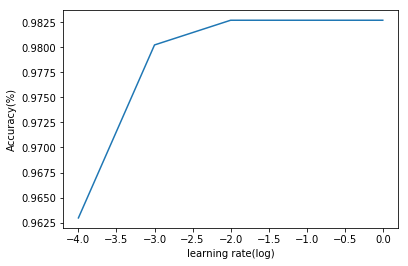
\includegraphics[width=0.6\textwidth]{pics/learning_rate.png}
	\caption{2-3 classifier accuracy versus learning rate}
\end{figure}

From the picture we can note that the learning rate of $10^{-2}$ actually achieve the best results.  For the following discussion, it is assumed that learning rate of $10^{-2}$ is used.

\subsection{Discussion}
\subsubsection*{(a)}
We learn our model by using 10\% holdout from the training set. During the training, the training data are divided into batch size of 32 minibatch before feed into the optimizer. 

With 400 epochs of training, we obtain the following result:
\begin{figure}[h]
	\begin{minipage}{0.48\textwidth}
	\centering
	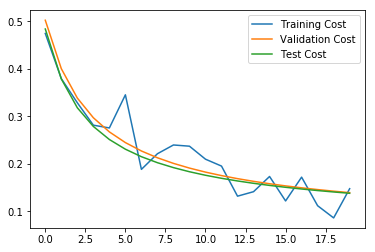
\includegraphics[width=\textwidth]{pics/2_3_loss.png}
	\caption{2-3 classifier loss function versus training epochs}
	\end{minipage}\hfill
	\begin{minipage}{0.48\textwidth}
	\centering
	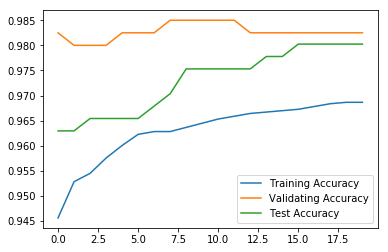
\includegraphics[width=\textwidth]{pics/2_3_accuracy.png}
	\caption{2-3 classifier accuracy function versus training epochs}
\end{minipage}
	
\end{figure}

Early stop is also implemented in our model, but since the holdout loss keeps decreasing, the training does not have an early stop this time. 

The holdout set does have a similar behavior as the test set. They exhibit highly similar values in terms of loss. It means that the holdout set is a good stand in for the testing set, which justifies the early stop method that prevents the model from overfitting. The reason why the results are so similar is quite obvious, the separation of the holdout set and the training set is random and the hold out set does not participate in the training procedure, which makes them as alien to the model as the testing set. 

\subsubsection*{(b)}
The results of the accuracy of the 2-3 classifier is shown in the figure. As observed, the hold out set has the highest accuracy, followed by the testing set and the training set. This may due to some special cases in the data.
The test accuracy for this model is 98.02\%.
\subsubsection*{(c)}
The same procedures are applied to 2-8 classifier. The test accuracy for this model is 96.10\%.
\begin{figure}[h]
	\begin{minipage}{0.48\textwidth}
		\centering
		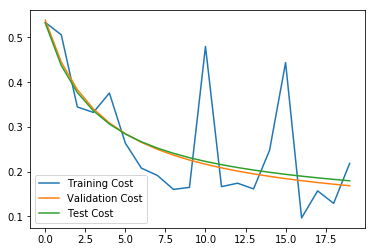
\includegraphics[width=\textwidth]{pics/2_8_loss.png}
		\caption{2-8 classifier loss function versus training epochs}
	\end{minipage}\hfill
	\begin{minipage}{0.48\textwidth}
		\centering
		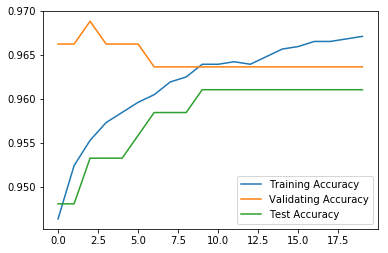
\includegraphics[width=\textwidth]{pics/2_8_accuracy.png}
		\caption{2-8 classifier accuracy function versus training epochs}
	\end{minipage}
\end{figure}

\subsubsection*{(d)}
We then display the weights from the two classifiers as well as their difference. 
\begin{figure}[h]
	\begin{minipage}{0.3\textwidth}
		\centering
		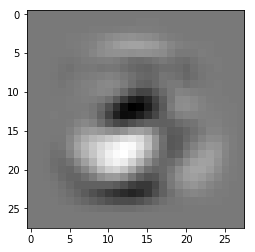
\includegraphics[width=\textwidth]{pics/2_3.png}
		\caption{Weights of 2-3 classifier}
	\end{minipage}\hfill
	\begin{minipage}{0.3\textwidth}
		\centering
		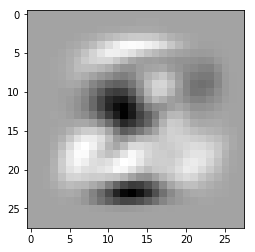
\includegraphics[width=\textwidth]{pics/2_8.png}
		\caption{Weights of 2-8 classifier}
	\end{minipage}\hfill
	\begin{minipage}{0.3\textwidth}
		\centering
		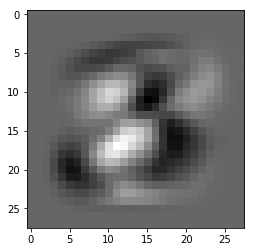
\includegraphics[width=\textwidth]{pics/3_8.png}
		\caption{difference between the two classifier}
	\end{minipage}
\end{figure}
We can actually interpret the classifier from the figures. For 2-3 classifier, the part that makes '2' a 2 is the right white part in the left bottom corner, basically the horizontal stoke of 2. And '3' is a 3 for the middle black part, and the bottom black part. Similar analysis can be made on the 2-8 classifier. The '8' is classifid to 8 when it has the black part in the top left corner, which 2 does not have. The difference of the weight is obtained by subtracting the weight of 2-8 from the weight of 2-3. We counter the weights of '2' in the difference. It can be use as a weight of 8-3 classifier, which outputs 1 when it is '8' and 0 when it is '3'. 
\newpage
\section{Regulation}
\subsection{Problem abstract}
Sometimes the regression model suffers from over fit, which reduces the generalization of the model. This can be improved by introducing regularization part to the loss function. With the cost function becoming \begin{align*}
J(w) = E(w) + \lambda C(w)
\end{align*}
 the loss function is penalized by the complexity of model parametrized by value $\lambda$. There are two major forms of regularization. 
 
 $L_1:$\begin{align*}
  C(w) = ||w||
  \end{align*}
 $L_2:$\begin{align*}
 C(w) = ||w||^2
 \end{align*}
\subsection{Discussion}
\subsubsection*{(a)} 
To derive the gradient descent of the two types of regularizations, we have 

$L_1$: \begin{align*}
\frac{d}{dw_j}C(w) = sgn(w_j) 
\end{align*}
$L_2$: \begin{align*}
\frac{d}{dw_j}C(w) = 2w_j 
\end{align*}
\subsubsection*{(b)} 
To figure out the best $\lambda$ to regularize the weight, we train our model against the lambda value of 0.0001, 0.001, 0.01, 0.1 and 1, and two types of regularization respectively.
\begin{figure}[h]
	\centering
	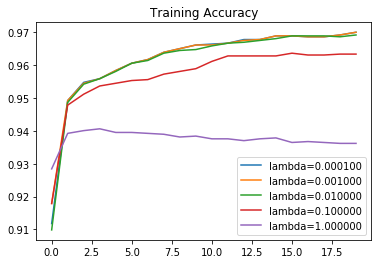
\includegraphics[scale = 0.7]{pics/lambda_train_1.png}
	\caption{L1 regularization. Model accuracy vs training epochs, with different values of lambda}
\end{figure}
\begin{figure}[h]
	\centering
	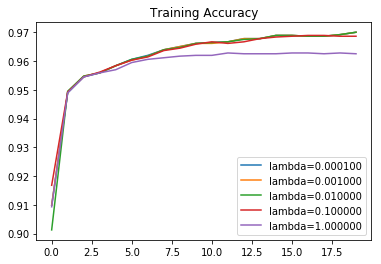
\includegraphics[scale = 0.7]{pics/lambda_train_2.png}
	\caption{L2 regularization. Model accuracy vs training epochs, with different values of lambda}
\end{figure}

From the figures we can observe, as lambda increases, the accuracy of training set decreases. It actually coincides with the intention to use regularization to penalize the overfitting of training set. As more regularization put on the training set, the model will not train into a state that over compliments the training data. Therefore it should not fit the training data that much when lambda goes up.

We also observe that the L1 regularization poses more penalty than the L2. It may be due to the fact that the absolute value of most of the weights here are far less than 1, making L1 regularization has a more significant effect than L2.
\subsubsection*{(c)}
To see the actual effect that regularization poses on weight, we plot the 2-norm of the weight versus the values of lambda. As observed, the weight keeps going down as the lambda goes up. It makes sense since the increase of lambda poses more penalty on the weight to keep the model free from large weights. 

\begin{figure}[h]
	\begin{minipage}{0.48\textwidth}
		\centering
		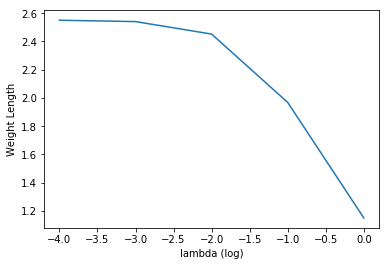
\includegraphics[width=\textwidth]{pics/weight_1.png}
		\caption{L1 regularization. Weight vector vs lambda}
	\end{minipage}\hfill
	\begin {minipage}{0.48\textwidth}
	\centering
		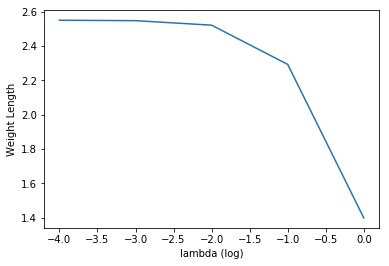
\includegraphics[width=\textwidth]{pics/weight_2.png}
		\caption{L2 regularization.  Weight vector vs lambda}
\end{minipage}
\end{figure}
\subsubsection*{(d)}
We then want to check the practical values of using regularization. By testing the regularized model on the testing data, we obtain the error rate of the model respectively for L1 and L2 regularization.
\begin{figure}[h]
	\begin{minipage}{0.48\textwidth}
		\centering
	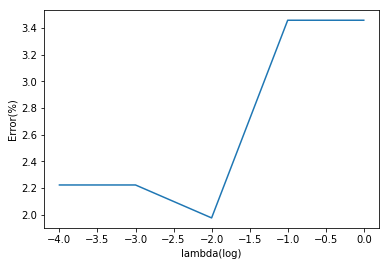
\includegraphics[width=\textwidth]{pics/lambda_test_1.png}
	\caption{L1 regularization. Test error versus lambda}
	\end{minipage}\hfill
	\begin {minipage}{0.48\textwidth}
	\centering
	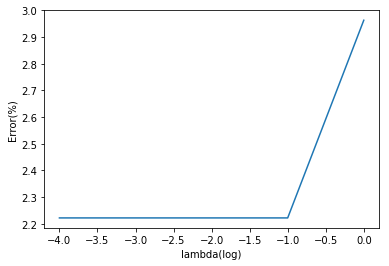
\includegraphics[width=\textwidth]{pics/lambda_test_2.png}
	\caption{L2 regularization. Test error versus lambda}
\end{minipage}
\end{figure}


As we can observed, the best lambda for L1 regularization is when $\lambda = 10^{-2}$, and $\lambda < 10^{-1}$ for L2. It makes sense that the regularization first helps with the generalization of the model that it prevents overfitting on the training data. Hence the error on the test set goes down when lambda goes up. Nonetheless, the increasing of lambda also impedes the pace of gradient descent that makes the model become under-trained. Hence we can observe an increase in error when lambda keeps going up.

The best lambda for our model is $\lambda=10^{-2}$ 
\subsubsection*{(e)}
\begin{figure}[h]
	\centering
	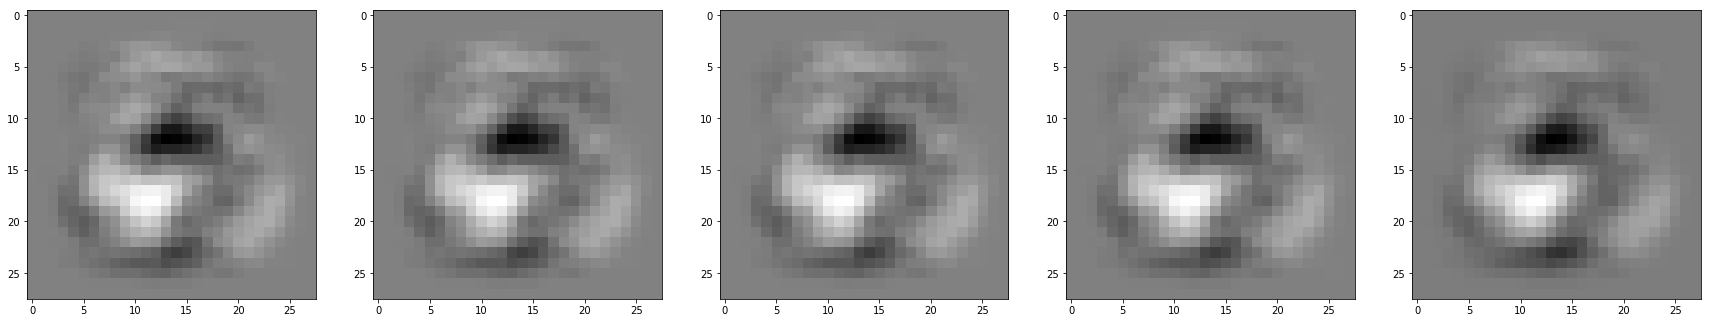
\includegraphics[width=\textwidth]{pics/weight_img.png}
	\caption{Weight images with different lambda. Lambda increases from left to right}
\end{figure}
Through the weight images, we can observe that with higher lambda, the weight image is actually more blurred than the one with lower lambda. There are mode granule details in images with lower lambda. This is may because the weights in lower lambda image can grow more freely than the one with higher lambda.
\newpage
\section{Softmax regression via gradient descent}
\subsection{Problem abstract}
The following section will focus on using the technique we have mention above to apply to all categories of hand-written digits. Softmax is the activation function we use in this application. It is an extension of the sigmoid function we used in Logistic Regression. Note that the softmax function is \begin{align*}
y_k^n =\frac{exp(a_k^n)}{\sum_{k'} exp(a_k'^n )}
\end{align*}

\subsection{Discussion}
\subsubsection*{(a)}
We first find the best lambda and regularization for the softmax model. 
\begin{figure}[h]
	\begin{minipage}{0.48\textwidth}
		\centering
		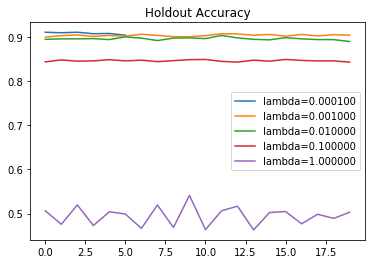
\includegraphics[width=\textwidth]{pics/softmax_reg_1.png}
		\caption{L1 regularization. Holdout  accuracy over training. Early stop enabled.}
	\end{minipage}\hfill
	\begin {minipage}{0.48\textwidth}
	\centering
	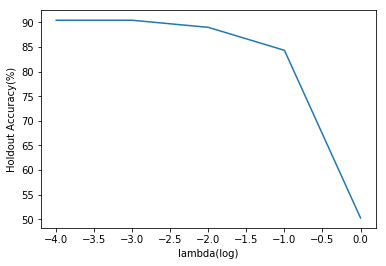
\includegraphics[width=\textwidth]{pics/softmax_reg_2.png}
	\caption{L1 regularization. Holdout accuracy vs lambda. Early stop enabled.}
\end{minipage}
\end{figure}
For L1 regularization, the holdout set has a highest accuracy when $\lambda=0.001$.
\begin{figure}[h]
	\begin{minipage}{0.48\textwidth}
		\centering
		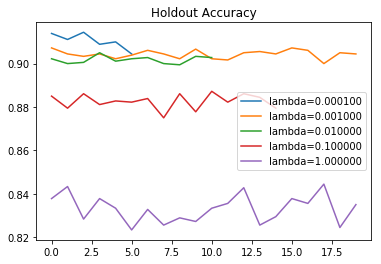
\includegraphics[width=\textwidth]{pics/softmax_reg_3.png}
		\caption{L2 regularization. Holdout  accuracy over training. Early stop enabled.}
	\end{minipage}\hfill
	\begin {minipage}{0.48\textwidth}
	\centering
	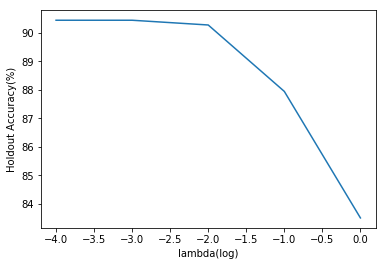
\includegraphics[width=\textwidth]{pics/softmax_reg_4.png}
	\caption{L2 regularization. Holdout accuracy vs lambda. Early stop enabled.}
\end{minipage}
\end{figure}
For L2 regularization, the holdout set has a highest accuracy when $\lambda=0.001$.

Note that the two kinds of regularization does not has a significant difference when $\lambda$ is low. However, as $\lambda$ increases in magnitude, the L1 regularization significantly impedes the accuracy, given its larger value compared to L2. We choose L2 for stabler result in general cases.
For the best case

\subsubsection{(b)}
Training accuracy 92.688889 %, Val accuracy 92.650000 %, Test accuracy: 93.600000 %
With L2 regularization and $\lambda=0.001$, we train the model to classify 10 hand written digits. The training loss is 0.4191, the holdout loss is 0.2726and the test loss is 0.2078.
\begin{figure}[h]
	\centering
	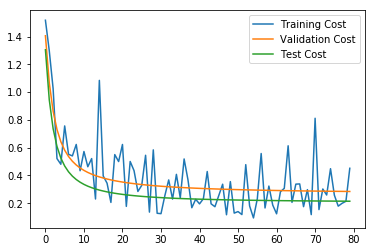
\includegraphics[width=0.7\textwidth]{pics/softmax_best_loss.png}
	\caption{The loss function plot versus every 20 training epochs for the trained softmax model. $\lambda =0.001$, L2 regularization, learning rate = 0.001. }
\end{figure}

\subsubsection{(c)}
With L2 regularization and $\lambda=0.001$, we train the model to classify 10 hand written digits. Training accuracy 92.688889 \%, val accuracy 92.650000 \%, and test accuracy: 93.600000 \%
\begin{figure}[h]
	\centering
	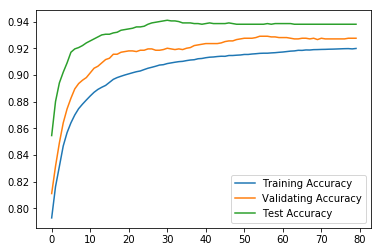
\includegraphics[width=0.7\textwidth]{pics/softmax_best_accuracy.png}
	\caption{The accuracy plot versus every 20 training epochs for the trained softmax model. $\lambda =0.001$, L2 regularization, learning rate = 0.001. }
\end{figure}

\subsubsection{(d)}
We plot the weight for each category and its corresponding average image in the training set in \ref{pic1}. 
\begin{figure}[thbp]\label{pic1}
	\begin{minipage}{0.48\textwidth}
		\centering
		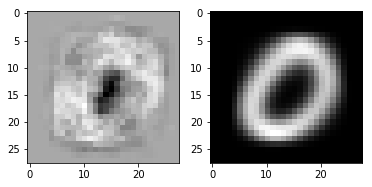
\includegraphics[width=\textwidth]{pics/0.png}
		\caption{Weight for category 0 and the average weight of 0 in training set}
	\end{minipage}\hfill
	\begin {minipage}{0.48\textwidth}
	\centering
	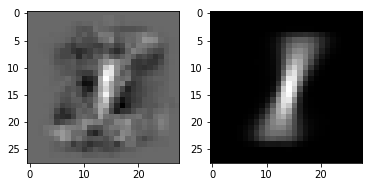
\includegraphics[width=\textwidth]{pics/1.png}
	\caption{Weight for category 1 and the average weight of 1 in training set}
\end{minipage}
	\begin{minipage}{0.48\textwidth}
		\centering
		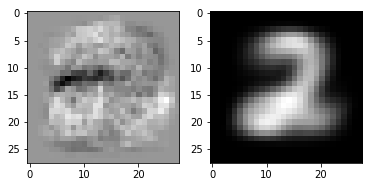
\includegraphics[width=\textwidth]{pics/2.png}
		\caption{Weight for category 2 and the average weight of 2 in training set}
	\end{minipage}\hfill
	\begin {minipage}{0.48\textwidth}
	\centering
	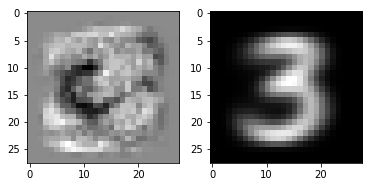
\includegraphics[width=\textwidth]{pics/3.png}
	\caption{Weight for category 3 and the average weight of 3 in training set}
\end{minipage}
	\begin{minipage}{0.48\textwidth}
		\centering
		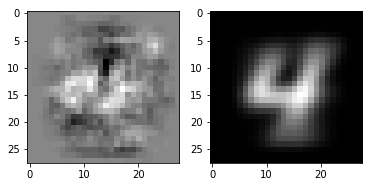
\includegraphics[width=\textwidth]{pics/4.png}
		\caption{Weight for category 4 and the average weight of 4 in training set}
	\end{minipage}\hfill
	\begin {minipage}{0.48\textwidth}
	\centering
	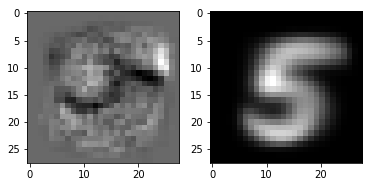
\includegraphics[width=\textwidth]{pics/5.png}
	\caption{Weight for category 5 and the average weight of 5 in training set}
\end{minipage}
	\begin{minipage}{0.48\textwidth}
		\centering
		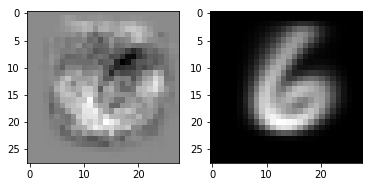
\includegraphics[width=\textwidth]{pics/6.png}
		\caption{Weight for category 6 and the average weight of 6 in training set}
	\end{minipage}\hfill
	\begin {minipage}{0.48\textwidth}
	\centering
	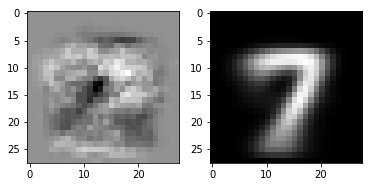
\includegraphics[width=\textwidth]{pics/7.png}
	\caption{Weight for category 7 and the average weight of 7 in training set}
\end{minipage}
	\begin{minipage}{0.48\textwidth}
		\centering
		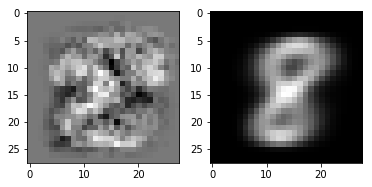
\includegraphics[width=\textwidth]{pics/8.png}
		\caption{Weight for category 8 and the average weight of 8 in training set}
	\end{minipage}\hfill
	\begin {minipage}{0.48\textwidth}
	\centering
	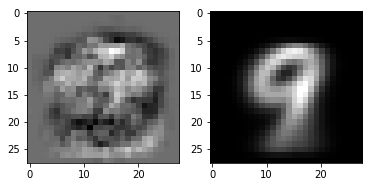
\includegraphics[width=\textwidth]{pics/9.png}
	\caption{Weight for category 9 and the average weight of 9 in training set}
\end{minipage}
\end{figure}

\subsection{Further Discussion}
\subsubsection{Adam Optimizer}
We use adam optimizer for updating parameters, this usually helps to get faster convergence. The following is the update rule we use:

\begin{equation*}
v = \beta_1 v + (1-\beta_1)\frac{\partial E}{\partial w}
\end{equation*}

\begin{equation*}
s = \beta_2 s + (1-\beta_2)(\frac{\partial E}{\partial w}^2)
\end{equation*}

\begin{equation*}
w = w - \alpha \frac{v}{\sqrt{s} + \epsilon}
\end{equation*}

\subsubsection{Mini-batch}
We also use mini-batch to increase update frequency and get faster convergence. In our program, we choose 32 as the batch size.


\newpage
\section{Summary}
To conclude, in this assignment, we first use logistic regression to discriminate digits of two categories. After experiment, we settle on the learning rate of 0.001 and the L2 regularization with parameter $\lambda = 0.001$ for our training task. We achieve a best result of 98.02\% accuracy on digits 2 and 3 and 96.10\% on 2 and 8. For the softmax task, we use a learning rate of 0.00001 and L2 regularization with  $\lambda = 0.001$, and achieve a accuracy of 93.60 \% on all ten categories.

From this assignment, we learn how to implement logistic and softmax regression. Through comparison and experimenting, we discover the effects of different parameters and the rationale behind each effect. 
\section{Contributions}
Fanjin Zeng is in charge of the derivation and logistic regression. He wrote the main frame of the codes for both logistic and softmax regression. 

Xinyue Ou is in charged of the regularization experimenting and softmax regression. He wrote part of the codes to help better illustrate the results we obtain in the model.


\section{References}
[1] Bishop, C. M., {\it Neural networks for pattern recognition}, Oxford: Oxford University Press, 2013.

\newpage
\section{Code}
\subsection{Logistic-Regression-MNIST.py}
\begin{lstlisting}[language=Python, breaklines]
	#!/usr/bin/env python3
	
	import numpy as np
	import matplotlib.pyplot as plt
	import struct
	import sys
	
	from utility import load_mnist_images, load_mnist_labels, sigmoid, \
	init_parameters, create_batch, extract_target_data, strictly_increasing
	
	
	def compute_cost(X, Y, w, b, lambd, regularized):
	    m = Y.shape[-1]
	    Z = np.dot(w, X) + b
	    A = sigmoid(Z)
	    cost =  - np.sum(Y * np.log(A) + (1-Y) * np.log(1-A)) / m
	
	    if regularized == 1:
	            cost += lambd * np.linalg.norm(w, 1) / m
	    elif regularized == 2:
	            cost += lambd * np.linalg.norm(w, 2) / m
	
	    return cost
	
	def logistic_propagate(X, Y, w, b, lambd, regularized):
	    m = Y.shape[-1]
	    Z = np.dot(w, X) + b
	    A = sigmoid(Z)
	
	    cost = compute_cost(X, Y, w, b, lambd, regularized)
	
	    dw = np.dot((A - Y), X.T) / m
	    db = np.sum((A - Y), axis=1, keepdims=True) / m
	
	    if regularized == 2:
	        dw += 2 * lambd * w / m
	    elif regularized == 1:
	        dw += lambd * np.sign(w) / m
	
	    grad = {'dw':dw, 'db':db}
	
	    return grad, cost
	
	
	def optimize(X, Y, w, b, learning_rate, lambd, regularized):
	    grad, cost = logistic_propagate(X, Y, w, b, lambd, regularized)
	
	    dw = grad['dw']
	    db = grad['db']
	
	    w -= learning_rate * dw
	    b -= learning_rate * db
	
	    return w, b, cost
	
	
	class LogisticRegression(object):
	
	    def __init__(self, n_feature, n_epoch, batch_size=32, learning_rate=0.001, lambd=0.01,\
	     regularized=2,  T=0., print_cost=False, print_period=20, record=False, record_period=20, early_stop=False, stop_step=3):
	        self.n_epoch = n_epoch
	        self.batch_size = batch_size
	        self.learning_rate = learning_rate
	        self.lambd = lambd
	        self.w, self.b = init_parameters(n_feature, 1)
	        self.cost = -1.
	        self.regularized = regularized
	        self.T = T
	
	        self.print_cost = print_cost
	        self.print_period = print_period
	        self.record = record
	        self.record_period = record_period
	        self.early_stop = early_stop
	        self.stop_step = stop_step
	
	
	    def fit(self, X, Y, holdout_X=None, holdout_Y=None, test_X=None, test_Y=None):
	        train = {'cost': [], 'accuracy': []}
	        val = {'cost': [], 'accuracy':[]}
	        test = {'cost':[], 'accuracy':[]}
	
	        for i in range(self.n_epoch):
	            X_batches, Y_batches, n_batch = create_batch(X, Y, self.batch_size)
	
	            for j in range(n_batch):
	                self.w, self.b, self.cost = optimize(X_batches[j], Y_batches[j], self.w, self.b, self.learning_rate, self.lambd, self.regularized)
	
	            self.learning_rate /= 1. + self.T
	
	            # record plot data, toggle by set record to True and set record period
	            if self.record and (i+1) % self.record_period == 0:
	                trainAcc = self.predict(X, Y)
	                train['cost'].append(self.cost)
	                train['accuracy'].append(trainAcc)
	
	                if holdout_X is not None:
	                    valCost = compute_cost(holdout_X, holdout_Y, self.w, self.b, self.lambd, self.regularized)
	                    valAcc = self.predict(holdout_X, holdout_Y)
	                    val['cost'].append(valCost)
	                    val['accuracy'].append(valAcc)
	
	                    if self.early_stop and (i+1) / self.record_period > self.stop_step and strictly_increasing(val['cost'][-self.stop_step:]):
	                        print('Early stop at %d epoch' % (i+1))
	                        break
	
	                if test_X is not None:
	                    testCost = compute_cost(test_X, test_Y, self.w, self.b, self.lambd, self.regularized)
	                    testAcc = self.predict(test_X, test_Y)
	                    test['cost'].append(testCost)
	                    test['accuracy'].append(testAcc)
	
	            # print cost, toggle by set print_cost to True and set print period
	            if self.print_cost and (i+1) % self.print_period == 0:
	                print('%d epoches cost: %f' % (i+1, self.cost))
	
	        return train, val, test
	
	
	    def predict(self, X, Y):
	        m = X.shape[-1]
	
	        Z = np.dot(self.w, X) + self.b
	        A = sigmoid(Z)
	
	        self.Y_p = (A > 0.5)
	        correct = (self.Y_p == Y)
	        self.accuracy = np.sum(correct) / m
	        return self.accuracy
	

\end{lstlisting}
\newpage
\subsection{Softmax-Regression-MNIST.py}
\begin{lstlisting}[language=Python, breaklines]
	#!/usr/bin/env python3
	
	import numpy as np
	import matplotlib.pyplot as plt
	import struct
	import sys
	
	from utility import load_mnist_images, load_mnist_labels, softmax, \
	one_hot_encoding, init_parameters, create_batch, strictly_increasing
	
	'''
	print(train_X.shape)    # n_feature * m_train
	print(test_X.shape) # n_feature * m_test
	print(train_Y.shape)    # 10 * m_train
	print(test_Y.shape) # 10 * m_test
	
	
	print(w.shape)  # 10 * n_feature
	print(b.shape)  # 10 * 1
	'''
	def compute_cost(X, Y, w, b, lambd, regularized):
	    m = Y.shape[-1]
	    Z = np.dot(w, X) + b
	    A = softmax(Z)
	    cost = - np.sum(Y * np.log(A)) / m
	
	    if regularized == 1:
	        cost += lambd * np.linalg.norm(w, 1) / m # L1 Regularization
	    elif regularized == 2:
	        cost += lambd * np.linalg.norm(w) / m  # L2 Regularization
	
	    return cost
	
	def softmax_propagate(X, Y, w, b, lambd, regularized):
	    m = Y.shape[-1]
	    Z = np.dot(w, X) + b
	    A = softmax(Z)
	
	    cost = compute_cost(X, Y, w, b, lambd, regularized)
	
	    dw = np.dot((A - Y), X.T) / m + 2 * lambd * w / m
	    db = np.sum((A - Y), axis=1, keepdims=True) / m
	
	    if regularized == 2:
	        dw += 2 * lambd * w / m
	    elif regularized == 1:
	        dw += lambd * np.sign(w) / m
	
	    grad = {'dw':dw, 'db':db}
	
	    return grad, cost
	
	def init_adam(w, b):
	    v = {}
	    s = {}
	
	    v['w'] = np.zeros((w.shape))
	    v['b'] = np.zeros((b.shape))
	
	    s['w'] = np.zeros((w.shape))
	    s['b'] = np.zeros((b.shape))
	
	    return v, s
	
	def adam_optimize(X, Y, parameters, learning_rate=0.001, lambd=0.01, beta1=0.9, beta2=0.999, epsilon=10**(-8), regularized=2):
	    w = parameters['w']
	    b = parameters['b']
	    v = parameters['v']
	    s = parameters['s']
	
	    grad, cost = softmax_propagate(X, Y, w, b, lambd, regularized)
	
	    dw = grad['dw']
	    db = grad['db']
	
	    v['w'] = beta1 * v['w'] + (1 - beta1) * dw
	    v['b'] = beta1 * v['b'] + (1 - beta1) * db
	
	    s['w'] = beta2 * s['w'] + (1 - beta2) * np.square(dw)
	    s['b'] = beta2 * s['b'] + (1 - beta2) * np.square(db)
	
	    w -= learning_rate * (v['w'] / (np.sqrt(s['w']) + epsilon))
	    b -= learning_rate * (v['b'] / (np.sqrt(s['b']) + epsilon))
	
	    parameters['w'] = w
	    parameters['b'] = b
	    parameters['v'] = v
	    parameters['s'] = s
	
	    return parameters, cost
	
	
	class SoftmaxRegression(object):
	
	    def __init__(self, n_feature, n_classes, n_epoch, batch_size=32, learning_rate=0.001,\
	     lambd=0.01, beta1=0.9, beta2=0.999, epsilon=10**(-8), regularized=2, T=0.,\
	     print_cost=False, print_period=20, record=False, record_period=20, early_stop=False, stop_step=3):
	        self.n_epoch = n_epoch
	        self.batch_size = batch_size
	        self.learning_rate = learning_rate
	        self.lambd = lambd
	        self.beta1 = beta1
	        self.beta2 = beta2
	        self.epsilon = epsilon
	        self.cost = -1.
	        self.regularized = regularized
	        self.T = T
	
	        w, b = init_parameters(n_feature, n_classes)
	        v, s = init_adam(w, b)
	        self.parameters = {'w':w, 'b':b, 'v':v, 's':s}
	
	        self.print_cost = print_cost
	        self.print_period = print_period
	        self.record = record
	        self.record_period = record_period
	        self.early_stop = early_stop
	        self.stop_step = stop_step
	
	    def fit(self, X, Y, holdout_X=None, holdout_Y=None, test_X=None, test_Y=None):
	        train = {'cost': [], 'accuracy': []}
	        val = {'cost': [], 'accuracy':[]}
	        test = {'cost':[], 'accuracy':[]}
	
	        for i in range(self.n_epoch):
	            X_batches, Y_batches, n_batch = create_batch(X, Y, self.batch_size)
	
	            for j in range(n_batch):
	                self.parameters, self.cost = adam_optimize(X_batches[j], Y_batches[j], self.parameters, \
	                self.learning_rate, self.lambd, self.beta1, self.beta2, self.epsilon, self.regularized)
	
	            self.learning_rate /= 1. + self.T
	
	            # record plot data, toggle by set record to True and set record period
	            if self.record and (i+1) % self.record_period == 0:
	                trainAcc = self.predict(X, Y)
	                train['cost'].append(self.cost)
	                train['accuracy'].append(trainAcc)
	
	                if holdout_X is not None:
	                    valCost = compute_cost(holdout_X, holdout_Y, self.parameters['w'], self.parameters['b'], self.lambd, self.regularized)
	                    valAcc = self.predict(holdout_X, holdout_Y)
	                    val['cost'].append(valCost)
	                    val['accuracy'].append(valAcc)
	
	                    if self.early_stop and (i+1) / self.record_period > self.stop_step and strictly_increasing(val['cost'][-self.stop_step:]):
	                        print('Early stop at %d epoch' % (i+1))
	                        break
	
	                if test_X is not None:
	                    testCost = compute_cost(test_X, test_Y, self.parameters['w'], self.parameters['b'], self.lambd, self.regularized)
	                    testAcc = self.predict(test_X, test_Y)
	                    test['cost'].append(testCost)
	                    test['accuracy'].append(testAcc)
	
	            # print cost, toggle by set print_cost to True and set print period
	            if self.print_cost and (i+1) % self.print_period == 0:
	                print('%d epoches cost: %f' % (i+1, self.cost))
	
	        return train, val, test
	
	
	    def predict(self, X, Y):
	        m = X.shape[-1]
	
	        w = self.parameters['w']
	        b = self.parameters['b']
	        Z = np.dot(w, X) + b
	        A = softmax(Z)
	
	        self.Y_p = np.argmax(A, axis=0)
	        Y_label = np.argmax(Y, axis=0)
	        correct = (self.Y_p == Y_label)
	
	        self.accuracy = np.sum(correct)/ m
	
	        return self.accuracy
	
\end{lstlisting}
\newpage
\subsection{utility.py}
\begin{lstlisting}[language=Python,breaklines]
	#!/usr/bin/env python3
	
	import numpy as np
	import struct
	import sys
	
	
	def load_mnist_images(path, max_images=sys.maxsize):
	    with open(path, 'rb') as f:
	        f.read(4)
	        n = int(struct.unpack('>i', f.read(4))[0])
	        n = min(max_images, n)
	        n_rows = int(struct.unpack('>I', f.read(4))[0])
	        n_cols = int(struct.unpack('>I', f.read(4))[0])
	        images = []
	        for i in range(n):
	            image = np.zeros((n_rows,n_cols), dtype=np.int16)
	            for r in range(n_rows):
	                for c in range(n_cols):
	                    image[r,c] = int(struct.unpack('>B', f.read(1))[0])
	            images.append(image)
	    return np.array(images)
	
	def load_mnist_labels(path, max_labels=sys.maxsize):
	    with open(path, 'rb') as f:
	        f.read(4)
	        n = int(struct.unpack('>i', f.read(4))[0])
	        n = min(max_labels, n)
	        labels = []
	        for i in range(n):
	            label = int(struct.unpack('>B', f.read(1))[0])
	            labels.append(label)
	    return np.array(labels)
	
	def extract_target_data(X, Y, target1, target2):
	    p1 = (Y == target1)
	    p2 = (Y == target2)
	    p = p1 | p2
	    x_target = X[:,p]
	    y_target = Y[p]
	    y_target = (y_target == target1)
	    y_target = np.expand_dims(y_target, axis=0)
	    return x_target, y_target
	
	def split_holdout(X, Y, holdout_ratio):
	    m = X.shape[-1]
	    permutation = np.random.permutation(m)
	    X_shuffle = X[:, permutation]
	    Y_shuffle = Y[:, permutation]
	    m_holdout = int(m * holdout_ratio)
	    return X[:,:-m_holdout], Y[:,:-m_holdout], X[:,-m_holdout:], Y[:,-m_holdout:]
	
	def strictly_increasing(L):
	    return all(x<y for x, y in zip(L, L[1:]))
	
	def sigmoid(x):
	    return 1. / (1 + np.exp(-x))
	
	def softmax(x):
	    z = np.exp(x)
	    z = z / np.sum(z, axis=0, keepdims=True)
	    return z
	
	def one_hot_encoding(labels, n_feature):
	    m = labels.shape[0]
	    encode = np.zeros((n_feature, m), dtype=int)
	    for i in range(m):
	        encode[labels[i], i] = 1
	    return encode
	
	def init_parameters(dim1, dim2, setZero=True):
	    if setZero:
	        w = np.zeros((dim2, dim1))
	    else:
	        w = np.random.randn(dim2, dim1) * 0.01
	
	    b = np.zeros((dim2, 1))
	    return w, b
	
	def create_batch(X, Y, batch_size):
	    m = X.shape[-1]
	    n_batch = int(m / batch_size)
	
	    X_batches = []
	    Y_batches = []
	
	    permutation = np.random.permutation(m)
	    X_shuffle = X[:, permutation]
	    Y_shuffle = Y[:, permutation]
	
	    for i in range(n_batch):
	        X_batch = X_shuffle[:, i * batch_size: (i+1) * batch_size]
	        Y_batch = Y_shuffle[:, i * batch_size: (i+1) * batch_size]
	        X_batches.append(X_batch)
	        Y_batches.append(Y_batch)
	
	    if m % n_batch != 0:
	        X_batch = X_shuffle[:, n_batch * batch_size:]
	        Y_batch = Y_shuffle[:, n_batch * batch_size:]
	        X_batches.append(X_batch)
	        Y_batches.append(Y_batch)
	        n_batch += 1
	
	    return X_batches, Y_batches, n_batch
	
\end{lstlisting}

\end{document}